\section{Binomische Formeln}
\label{binomisch}
Autor: Katja Matthes
%%%%%%%%%%%%%%%%%%%%%%%%%%%%%%%%%%%%%%%%%%%%%%%%%%%%%%%%%%%%%%
%%%Definition
%%%%%%%%%%%%%%%%%%%%%%%%%%%%%%%%%%%%%%%%%%%%%%%%%%%%%%%%%%%%%%
\subsection{Definition}
Die Binomischen Formeln sind Formeln zur Darstellung und zum Lösen von Quadrat-Binomen. Sie erleichtern das Ausmultiplizieren von Klammer"-aus"-drü"-ck"-en und erlauben Term-Umformungen von bestimmten Summen und Differenzen in Produkte. Dies stellt sehr oft die einzige Lösungsstrategie bei der Vereinfachung von Bruchtermen, beim Radizieren von Wurzeltermen sowie Logarithmenausdrücken dar.
%%%%%%%%%%%%%%%%%%%%%%%%%%%%%%%%%%%%%%%%%%%%%%%%%%%%%%%%%%%%%%
%%%Formeln
%%%%%%%%%%%%%%%%%%%%%%%%%%%%%%%%%%%%%%%%%%%%%%%%%%%%%%%%%%%%%%
\subsection{Formeln}
%%%%%%%%%%%%%%%%%%%%%%%%%%%%%%%%%%%%%%%%%%%%%%%%%%%%%%%%%%%%%%
%%%1. Binomische Formeln
%%%%%%%%%%%%%%%%%%%%%%%%%%%%%%%%%%%%%%%%%%%%%%%%%%%%%%%%%%%%%%
\subsubsection{Erste binomische Formel}
	\[(a + b)^2 = a^2 + 2ab + b^2\]
Die erste binomische Formel kann wie im folgenden Bild dargestellt werden:
\begin{center}
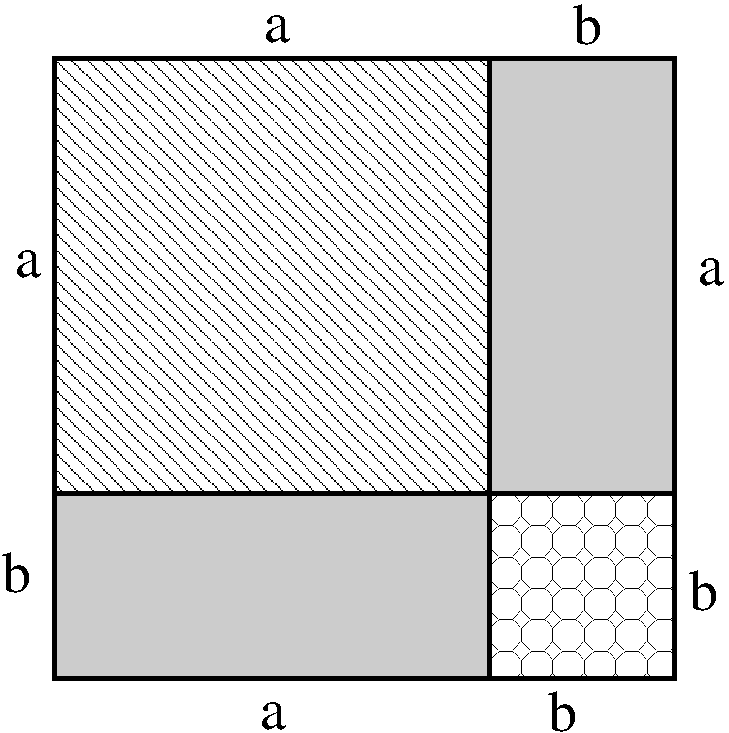
\includegraphics[height=3cm]{img/binF1.pdf}
\end{center}
Die Fläche eines Quadrates entspricht seiner Seitenlänge zum Quadrat. In der Abbildung beträgt die Seitelänge des Quadrats $ (a+b) $. Dementsprechend ist der Flächeninhalten des gesamten Quadrates $ (a+b)^2 $.

Die gleiche Fläche entsteht auch, indem ein schraffiertes Quadrat (Fläche: $ a^2 $), zwei graue Rechtecke (Fläche: $ 2\cdot ab $) und ein gekringeltes Quadrat (Fläche: $ b^2 $) zusammen gelegt werden. Es ergibt sich also folgende Legende: 
\begin{center}
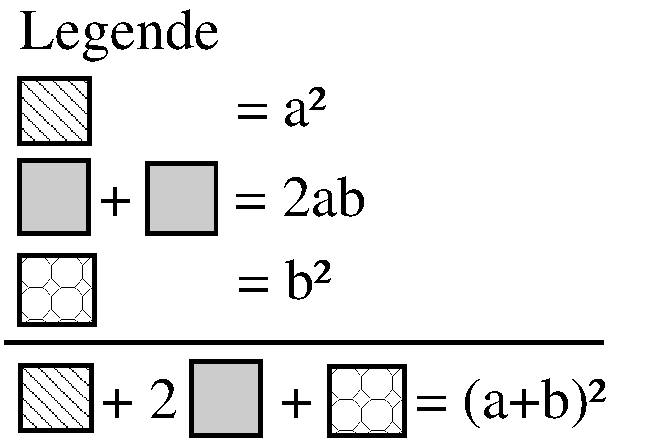
\includegraphics[height=2cm]{img/binF1legende.pdf}
\end{center}
%%%%%%%%%%%%%%%%%%%%%%%%%%%%%%%%%%%%%%%%%%%%%%%%%%%%%%%%%%%%%%
%%%2. Binomische Formeln
%%%%%%%%%%%%%%%%%%%%%%%%%%%%%%%%%%%%%%%%%%%%%%%%%%%%%%%%%%%%%%
\subsubsection{Zweite binomische Formel}
	\[(a - b)^2 = a^2 - 2ab + b^2\]
Die zweite binomische Formel kann durch folgende Abbildung veranschaulicht werden:
\begin{center}
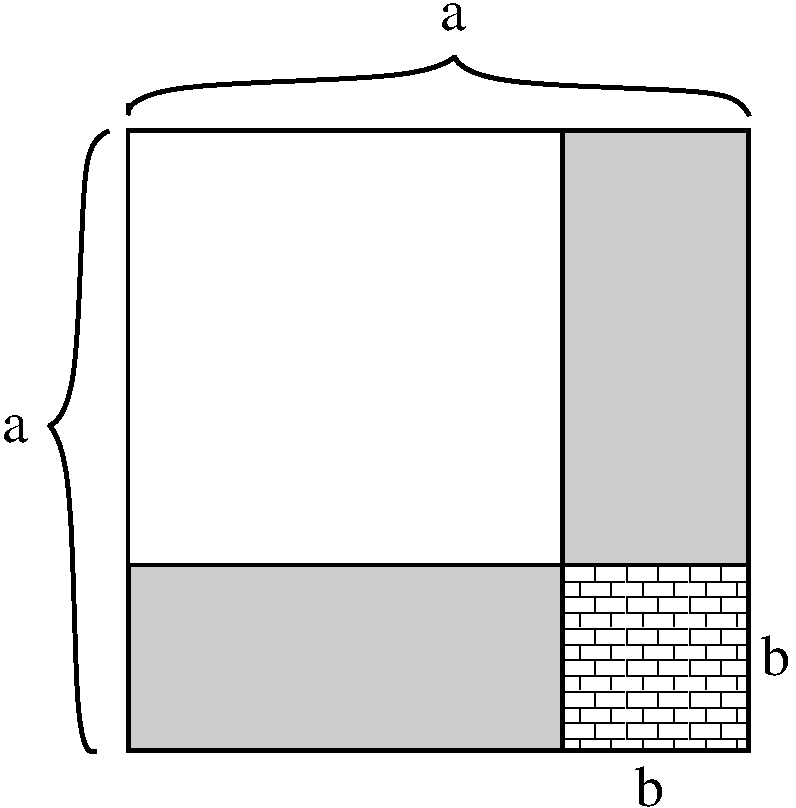
\includegraphics[height=3cm]{img/binF2.pdf}
\end{center}
Gesucht ist der Flächeninhalt des wei\ss en Quadrats: $(a-b)^2$. Das gesamte Quadrat in der Abbildung hat eine Fläche von $ a^2 $. Zur Berechnung stehen zwei weitere Flächen zur Verfügung: Das gekachelte Quadrat besitzt alleine einen Flächeninhalt von $b^2$ und zusammen mit einem grauen Rechteck jeweils einen Flächeninhalt von $ ab $. Um die gesuchte Fläche zu erhalten, können von dem gesamten Quadrat zunächst die zwei grauen Rechtecke entfernt werden, indem $ 2\cdot ab $ abgezogen werden (also: $ -2\cdot ab $). Dadurch wird das gekachelte Quadrat jedoch ein mal zuviel entfernt, so dass es wieder hinzuaddiert werden muss ($+b^2$). Daraus ergibt sich folgende Legende:
\begin{center}
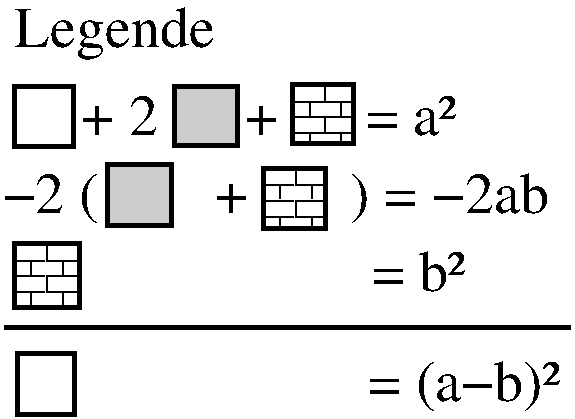
\includegraphics[height=2cm]{img/binF2legende.pdf}
\end{center}
%%%%%%%%%%%%%%%%%%%%%%%%%%%%%%%%%%%%%%%%%%%%%%%%%%%%%%%%%%%%%%
%%%3. Binomische Formeln
%%%%%%%%%%%%%%%%%%%%%%%%%%%%%%%%%%%%%%%%%%%%%%%%%%%%%%%%%%%%%%
\subsubsection{Dritte binomische Formel}
	\[(a + b)(a - b) = a^2 - b^2\]
Die dritte binomische Formel kann mit Hilfe der beiden folgenden Bilder erklärt werden:
\begin{center}
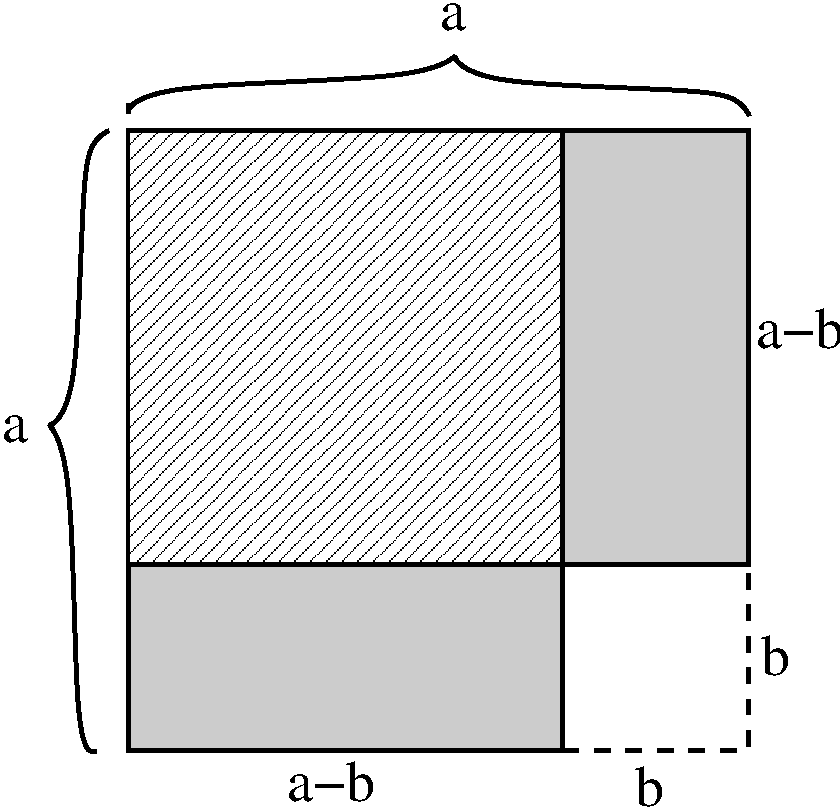
\includegraphics[height=3cm]{img/binF3a.pdf}
\end{center}
Gesucht ist die Fläche, die aus dem schraffierten Quadrat und den beiden grauen Rechtecken besteht. Am einfachsten erhalten wir diese, indem wir (wieder) vom gesamten Quadrat (Fläche: $a^2$) das kleine wei\ss e Quadrat (Fläche: $b^2$) abziehen. Allerdings können wir die Flächen auch so anordnen, dass das folgende Bild entsteht.
\begin{center}
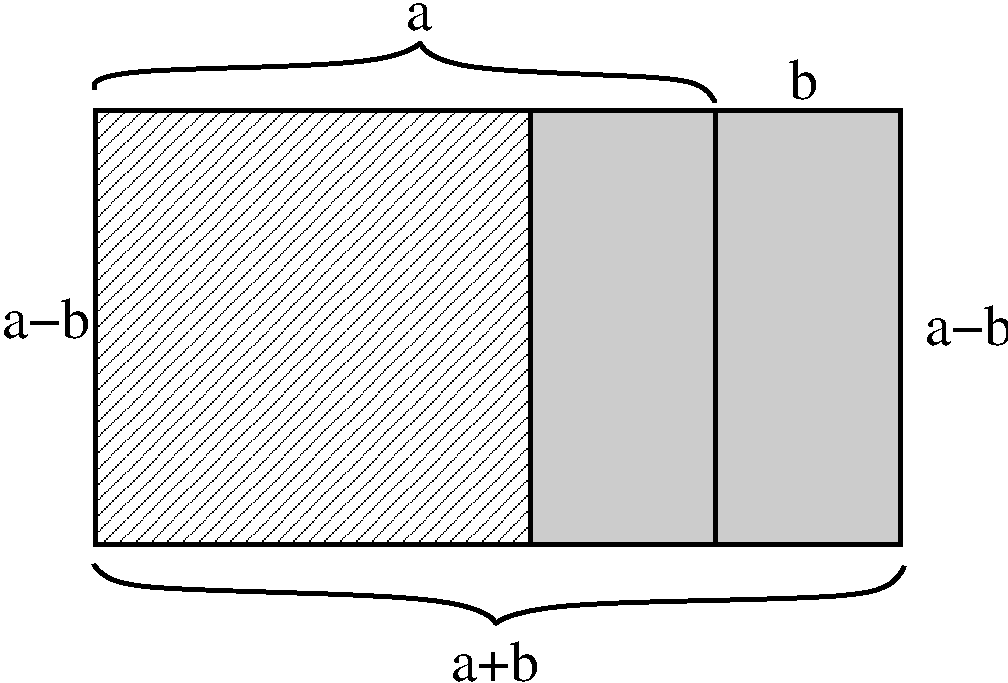
\includegraphics[height=3cm]{img/binF3b.pdf}
\end{center}
Die Fläche eines Rechtecks entspricht dem Produkt seiner Seitenlängen, hier $(a+b)$ und $(a-b)$. Daraus ergibt sich folgende Legende:
\begin{center}
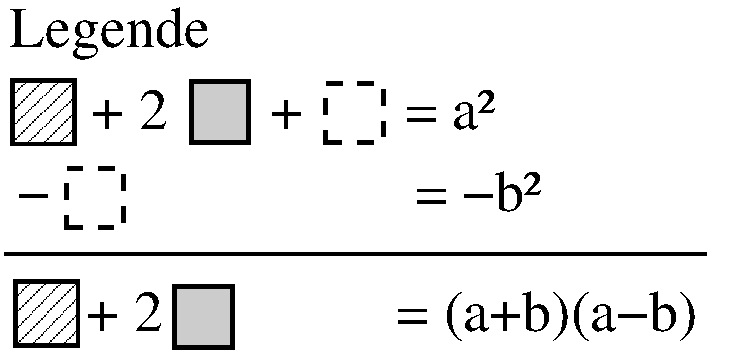
\includegraphics[height=2cm]{img/binF3legende.pdf}
\end{center}
%%%%%%%%%%%%%%%%%%%%%%%%%%%%%%%%%%%%%%%%%%%%%%%%%%%%%%%%%%%%%%
%%%Literatur
%%%%%%%%%%%%%%%%%%%%%%%%%%%%%%%%%%%%%%%%%%%%%%%%%%%%%%%%%%%%%%

%%%%%%%%%%%%%%%%%%%%%%%%%%%%%%%%%%%%%%%%%%%%%%%%%%%%%%%%%%%%%%
%%%Aufgaben
%%%%%%%%%%%%%%%%%%%%%%%%%%%%%%%%%%%%%%%%%%%%%%%%%%%%%%%%%%%%%%
\subsection{Aufgaben}

\subsubsection{Aufgabe 1}
Wende die binomischen Formeln zur Vereinfachung an.
\begin{enumerate}
\begin{multicols}{2}
	\item \quad $ (4x + 3y^3)^2 $
	\item \quad $ -(x^4-2)^2 $
	\item \quad $ (x^2-x^3)(x^2+x^3) $
	\item \quad $ (3x^2+2t)^2 $
	\item \quad $ -\frac{1}{2}(x^2-4)^2 $
	\item \quad $ \left(-\frac{1}{2}(x^2-4)\right)^2 $
	\item \quad $ x^2y^2(x^4+2x^2y+y^2) $
\end{multicols}
\end{enumerate}

\pagebreak
\subsubsection{Aufgabe 2}
Vereinfache. Verwende dabei die binomischen Formeln.
\begin{enumerate}
\begin{multicols}{2}
	\item \quad $ (x-3)^n \cdot (x+3)^n $
	\item \quad $ \frac{(a^2-b^2)^3}{(a-b)^3} $
	\item \quad $ \frac{(4-x^2)^n}{(2-x)^n} $
	\item \quad $ \frac{(c-1)^{n-1}}{(c^2-1)^{n-1}} $
	\item \quad $ \frac{(a^{2n}-b^{2n})^2}{(a^n-b^n)^2} $
	\item \quad $ (a^3 - ab^2)(a+b)^2 $
	\item \quad $ \frac{[(x-y)^2]^k}{(x^2-y^2)^k} $
	\item \quad $ (a+b)^4(a-b)^4(a^2-b^2)^5 $
\end{multicols}
\end{enumerate}

\subsubsection{Aufgabe 3}
Faktorisiere/Schreibe als Produkt.
\begin{enumerate}
\begin{multicols}{2}
	\item \quad $ (3x-6)\left(\frac{1}{4}x^2 - x + 1\right) $
	\item \quad $ a^2 - 2a^3 + a^4 $
	\item \quad $ 3a^3 - 12a^9 $
	\item \quad $ x^4 - a^2 $
	\item \quad $ 3-x^2 $
	\item \quad $ x^{2n} + 4x^n + 4 $
	\item \quad $ x^{n+2} -6x^{n+1} + 9x^n $
	\item \quad $ e^{2x}-1 $
	\item \quad $ x^2e^x + 2xe^x +e^x $
\end{multicols}
\end{enumerate}

\subsubsection{Aufgabe 4}
Vereinfache.
\begin{enumerate}
\begin{multicols}{2}
	\item \quad $ \frac{a^3+2a^2b+ab^2}{(a+b)^2} $
	\item \quad $ \frac{a^4-a^2b^2}{ab-a^2} $
	\item \quad $ \frac{t^3+6t^2+9t}{t^2-9} $
	\item \quad $ \frac{x^{2n}-10x^n+25}{x^{2n}-25} $
	\item \quad $ \frac{x^6-t^2}{x^4+tx} $
	\item \quad $ \frac{x^{n+3}-x^{n+1}}{x^{n+1}+x^n} $
	\item \quad $ \frac{(x^2+8xy+16y^2)}{(2x-3y)^{-2}} : \frac{x^2-16y^2}{2x-3y} $
	\item \quad $ \frac{4t^2-4}{t^2+2t+1} $
	\item \quad $ \frac{x^{n-1}-x^n}{x^n-x^{n+2}} $
	\item \quad $ \frac{2(a^2+b^2)^2}{a^5-ab^4} $
	\item \quad $ \frac{x^4-x^3}{x^4-x^2} $
	\item \quad $ \frac{x^3y-xy^5}{x^3y^2-x^2y^4} $
	\item \quad $ \frac{am-an+bm-bn}{a^2-b^2} $
\end{multicols}
\end{enumerate}

\pagebreak
\subsubsection{Aufgabe 5}
Multipliziere aus und vereinfache.
\begin{enumerate}
\begin{multicols}{2}
	\item \quad $ (e^x+e^{-x})^2 $
	\item \quad $ (a^2-a^{-2})^2 $
	\item \quad $ (x^{-2}-3x)(x^{-2}+3x) $
	\item \quad $ (2^{-x}+2^x)(2^{-x}-2^x) $
\end{multicols}
\end{enumerate}

\subsection{Aufgabe 6}
Vereinfache/Fasse zusammen.
\begin{enumerate}
\begin{multicols}{2}
	\item \quad $ \frac{e^{2x}-e^{-2x}}{e^x-e^{-x}} $
	\item \quad $ \left(\frac{x-y}{a-b}\right)^5 \cdot \left(\frac{x-y}{5}\right)^{-2} \cdot \frac{(a-b)^2}{(x^2-y^2)} $
\end{multicols}
\end{enumerate}



